%!TEX root=document.tex

\section{Utility Metrics: Discussion}
\label{sec:discussion}
We now discuss and evaluate various aspects of our choice of utility metrics,
including:

\noindent {\it (a) Distance Functions.} We evaluate the final results on
using different distance functions for measuring deviation.

\noindent {\it (b) General Utilities.} We describe how our 
techniques can be used to capture a variety of other important aspects
for visualization recommendation beyond deviation. 

\noindent {\it (c) \SeeDB's Capabilities.} We study how
effective \SeeDB is at capturing
different distance functions and general utility metrics. We compare two
metrics to EMD and study impact on:
{\it (i)} performance; 
{\it (ii)} accuracy when pruning optimizations are employed.


We summarize our findings below.
\papertext{Details can be found in the technical report~\cite{seedb-tr}.}
\begin{denselist}
\item {\em (a)} The choice of distance function between Jenson-Shannon divergence (J-S), Euclidean distance, Kullback–Leibler (K-L) divergence
and EMD is not critical: the first three distance functions lead
to results that largely
agree with EMD in the visualization ordering. For instance, the
first three distance functions output 3 out of EMD's top-5 visualizations 
in their top-5, and
two out of three distance functions output 4 out of EMD's top-5 visualizations in their top-5.
\srm{Note the dataset that was used here.}
\item {\em (b)} We developed a generalized utility metric
that captures deviation from the baseline ({\it deviation}),
historical data ({\em history}),
variation in and distribution of the data itself ({\it data distribution}),
types and properties of the different attributes in the dataset ({\it metadata}), 
visual qualities of the visualization ({\it aesthetics}),  
past history of interactions with this user and other users ({\it user preferences}), and,
to a limited extent,
meaning and relative importance of attributes in the data ({\it semantics}).
%We have extended \SeeDB to support this generalized utility metric. 
\item {\em (c)} We evaluated EMD, the Euclidean distance, and MAX\_DIFF
(a general utility metric that captures the difference between the largest
and second largest aggregate group) within \SeeDB and found that
all three utility measures perform similarly in terms of performance 
(i.e., they lead to similar gains via our optimizations),
without sacrificing accuracy. 
\end{denselist}

\techreport{
\subsection{Distance Functions}
\label{sec:diff_dist_funcs}
By default, \SeeDB uses Earth Movers Distance (EMD) 
to compute distance between
the target and reference probability distributions.
However, as mentioned in Section \ref{sec:problem_statement}, 
other distance functions 
such as Euclidean distance, K-L divergence and J-S divergence 
may also be used in place of EMD. 
Note that these are all {\em consistent distance functions},
like we described in Section~\ref{sec:pruning_opt}.

We applied each of these distance functions---Euclidean,
K-L divergence, and J-S divergence---to 
our test datasets (\agp{which?}) and compared
the resulting recommendations orders to that of EMD. 
We found that for the top-$5$ visualizations
output by EMD, 
all three distance functions
output 3 out of 5 visualizations in their top-5, 
whereas two of three distance functions 
output 4 out of 5 visualizations in their top-5.
Similarly, for $k$=10, 
all three distance functions output 6 out of the top-10 visualizations
output by EMD in their top-10, while two of three distance functions
output 9 out of the top-10 visualizations output by
EMD in their top-10.

Thus, we find a high degree of agreement on the 
top visualizations according to multiple distance functions.
We see similar results for the lowest utility visualizations as well. 
For the bottom-$5$ visualizations output by EMD, 
all three distance functions output 3 out of 5 in their top-5, 
and two of three distance functions output 4 out of 5 in their top-5.
These results indicate that the choice of specific distance 
function measuring deviation is not
critical; the above functions produce similar 
orderings of visualizations.

\subsection{General Utility Metrics}\label{sec:gen_util}

% In this section we prove that our sampling 
% algorithms converge, and then describe our generalized
% distance metric.

In addition to deviation, there are several other aspects
or {\em dimensions} that need to be taken into account
in order to make data-driven recommendations even more powerful.
Here, we list these dimensions, and then describe how 
we augment \SeeDB to incorporate these dimensions.
A full exploration of these dimensions
and their relative importance is left as future work.
  
The dimensions that determine the quality of a visualization recommendation
include:
  \begin{inparaenum}
  \item deviation from the baseline ({\it deviation}),
  \item historical data ({\em history}),
  \item variation in and distribution of the data itself ({\it data distribution}),
  \item types and properties of the different attributes in the dataset ({\it metadata}), 
\item visual qualities of the visualization ({\it aesthetics}),  
\item past history of interactions with this user and other users ({\it user preferences}), and 
\item meaning and relative importance of attributes in the data ({\it semantics}). 
\end{inparaenum}
We now describe how \SeeDB can be augmented to support these dimensions
within the utility metric.

First, consider an extension of the utility metric  
$U (V_i)$ denoted as $f_D (V_i)\ =\ w_d \times S_d + w_h \times S_h + w_l  \times S_l$.
Here, the first component corresponds to the utility  
from Section~\ref{sec:problem_statement}
so that $S_d = S ( P[V_i (D_Q)],$ $P[V_i (D_R)] )$ 
takes into account the {\em deviation} between the target data and the reference (item 1 above).
We can use the same distance function $S$ to also capture utility based on historical context. 
For instance, let $S_h = S ( P[V_i (D_Q)], $ $P[V_i (D_C)] )$ where
$P[V_i (D_C)]$ refers to the typical value of the distribution 
$P[V_i (D_Q)]$, given historical data.
For instance, when $V_i$ refers to sales of a particular chair in 
Boston, $V_i(D_C)$ could be sales of that chair in Boston for the past 10 years.
This measure would then allow us to identify whether the value for particular sales is 
deviating significantly from past patterns and is therefore interesting (item 2 above).
Finally, we can also use the distance function to capture local trends.
For instance, let $S_l = S ( P[V_i (D_Q)], P'[V_i (D_Q)] )$ where
$P'[V_i (D_Q)]$ refers to the distribution $P$, but shifted slightly.
For instance, if the sensor readings in the last five minutes differ greatly
for current readings, the utility of $V_i$ would be high.
This component can capture
the amount of rapid local changes that have happened
within the distribution corresponding to $P[V_i (D_Q)]$ (item 3 above).


Next, we turn to the question of incorporating other recommendation dimensions into our utility 
metric, beyond items 1--3 above that are all distribution-based.
Consider the following form of a generalized utility metric:
$$ U (V_i) = f_{MA}(V_i) \times f_P (V_i) \times f_D (V_i)$$
Let $f_D (V_i)$ be the utility function measuring distribution-based utility of $V_i$ (items 1---3).
We can then augment $f_D (V_i)$ with $f_{MA}(V_i)$ and $f_P (V_i)$ capturing metadata  and aesthetics (item 4 and 5), and user preferences (item 6) respectively.
For instance, $f_{MA}(V_i)$ can capture best-practices about 
visualization and output a  value accordingly.
Similarly, let $f_P (V_i)$ be a function that models the users' preference towards seeing visualization $V_i$.
This function can take into account past user history at both the individual and global levels.
For instance, if the analyst typically looks at sales over time, $f_P (V_i)$ for sales over time
may be high.
Similarly, if sales is a popular attribute across all data analysts, $f_P (V_i)$ could be large for
a $V_i$ that depicts sales.
We can also think of $f_P (V_i)$ as capturing in a limited way semantics 
that can be mined from previous user interactions.
We note however that semantics (item 7 above) is one dimension that an automated 
recommendation system will not be able to capture fully.

In terms of the visualization recommendations, 
we find that $f_{MA}(V_i)$ and $P (V_i)$ are independent
of the data distribution.
Once a user poses a query, we can merely reuse previously 
computed values for these functions while
making the recommendation.
For \SeeDB, these functions amount merely to constants 
in the utility function $U (V_i)$ that would assign weights to each view.
Thus, in this form, \SeeDB has been extended to 
incorporate other recommendation dimensions into
the utility metric without any changes to the \SeeDB framework.



\begin{figure}[h]
	\centering
	\vspace*{-10pt}
	\begin{subfigure}{0.48\linewidth}
		\centering
		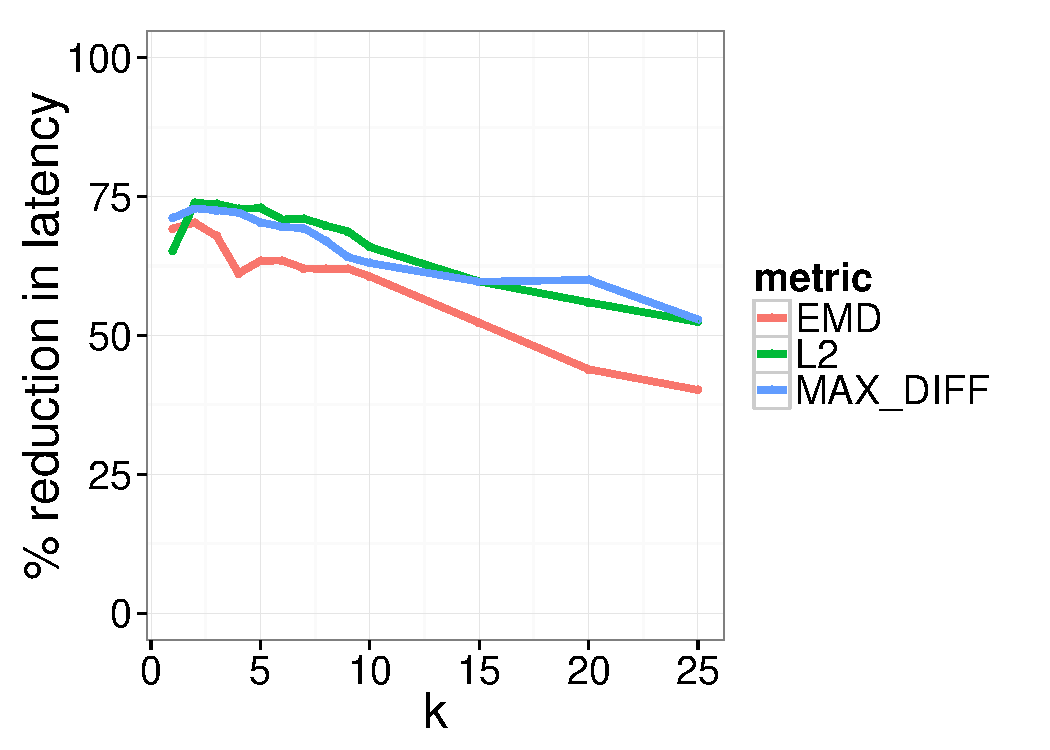
\includegraphics[width=4.4cm] {Images/in_memory_diff_metrics_latency.pdf}
		\vspace{-15pt}
		\caption{Latency}
		\label{fig:dist_latency}
	\end{subfigure}
	\begin{subfigure}{0.48\linewidth}
		\centering
		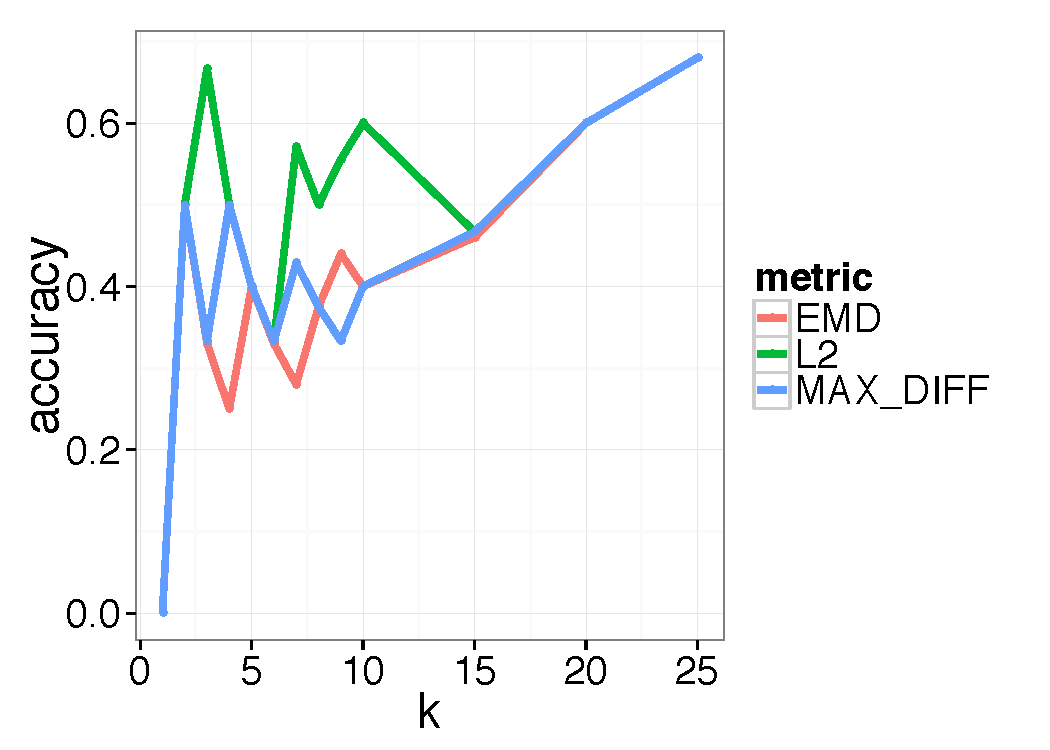
\includegraphics[width=4.4cm] {Images/in_memory_diff_metrics_accuracy.pdf}
		\vspace{-15pt}
		\caption{Accuracy}
		\label{fig:dist_accuracy}
	\end{subfigure}
	\vspace{-10pt}
\caption{Latency and Accuracy for different Distance Functions}	
		\vspace{-10pt}
\end{figure}


\subsection{Performance and Accuracy of {\large \SeeDB}}
In Section \ref{sec:pruning_opt}, we described the 
two pruning strategies used by \SeeDB
to rapidly discard low-utility views.
As seen in Section \ref{sec:experiments}, 
our strategies work well for the EMD-based 
utility metric.

Now, given that \SeeDB can support other
distance functions (Section~\ref{sec:diff_dist_funcs})
or general utility metrics (Section~\ref{sec:gen_util}),
we now focus on evaluating whether \SeeDB's optimizations
translate to gains on these other utility metrics.
We consider two other utility metrics
(a) Euclidean distance (L2): like EMD,
this is a deviation-based utility metric.
(b) Max deviation (MAX\_DIFF): this metric
measures the maximum deviation between
the highest aggregate, and the second highest
aggregate. This metric would, for example, score
visualization Figure~\ref{fig:huhi} very highly.


In Figure~\ref{fig:dist_latency}, we plot the reduction 
in latency for these metrics,
and in Figure~\ref{fig:dist_accuracy}, we plot the
accuracy, both as a function of $k$.
The results indicate that in all cases,
the reduction of latency is significant,
and is similar between EMD, L2 and MAX\_DIFF.
At the same time, the accuracy variation between 
EMD, L2, and MAX\_DIFF is also similar
(slight variations can be attributed to random noise).

These results indicate that \SeeDB is capable of
providing similar performance improvements on other
utility measures. 

\agp{This isn't very flattering...}
}%techreport

\if{0}
We now discuss the generality of our pruning techniques 
for other distance functions, and even other
utility metrics that uses the underlying data distribution in some way (not based on deviation).

% We define the set of utility metrics for which our pruning strategies work and provide intuition
% for why the strategies hold.

At the highest level, the goal of \SeeDB is to {\em estimate} for each visualization $V_i$, 
the value of its utility $U(V_i)$, however that utility may be defined.
In statistical terms, $U(V_i)$ is the {\em parameter} and the quantity we use to estimate the
utility is our {\em estimator}.
In our deviation-based metric (say using EMD), the parameter is the value of EMD on the full
dataset and our estimator is the mean value of EMD obtained from a sample of the data.
A {\em consistent estimator}~\cite{consistent_estimator} is an estimator having the property 
that as the size of the sample increases, estimates from the estimator tend towards the value 
of the parameter. \mpv{maybe a formula for consistent estimators}

With these definitions, we can define the set of utility metrics handled by CI and MAB as follows:
\begin{lemma}
Let $\mathcal{U}$ be any data-distribution based utility metric defined on a set of visualizations $\{
V_1 \ldots V_n\}$. Then the pruning strategies CI or MAB can correctly identify (upto some $\delta$) the 
$k$ visualizations with the highest values of $\mathcal{U}$ if and only if $\mathcal{U}$ has a consistent 
estimator $\mathcal{E}_C$ and $\mathcal{E}_C$ is used to compute utility estimates for CI or MAB.
\end{lemma}

The intuition behind this lemma is that {\em so long as the utility metric (and estimator) are such that
the estimates improve with increasing sample sizes}, the pruning performed by CI and MAB will have low
error rate.
At each phase, our pruning strategies can be thought of as operating on samples of increasingly larger
sizes, their estimates tending towards the value of the true utility.
As a consequence, the views that are pruned have (almost) as high accuracy as if the sample was used to
return the top-$k$ results.
Moreover, our strategies become increasingly accurate in subsequent phases.
\mpv{we perform strictly better than an algorithm than takes a sample of size = size of first phase1 and
returns top-$k$ from it.}

A rigorous proof of error bounds is outside the scope of this work.
We expect that a majority of potential data-driven utility metrics are, in fact, well-behaved with respect to 
our techniques.
Prior work has shown that sample means (utility mean for CI and MAB) is in fact a consistent estimator for
population mean (true utility)\cite{mean_is_consistent}.
Other metrics that fit our criterion include deviation-based techniques that use distance functions other than 
EMD to measure distance between distributions, utility based on maximum difference in distribution, 
and metrics that measure whether there is an outlier in the visualization.
There are of course (unrealistic) edge cases, e.g. utility is equal to a specific value in the last tuple scanned, that
do not have consistent estimators and cannot be handled by our pruning technique.

We empirically validate our lemma by testing our pruning strategy on other utility metrics. 
These metrics were: (1) Deviation using Euclidean distance; (2) Max deviation; (3) a Non-consistent
estimator.
Figure \ref{} shows the results of our experiments. 
We find that both our pruning strategies perform well for EUC and MAX\_DEV whereas they perform
poorly for NC.
\fi






% Let $f_{MA}(V_i)$ be a function that captures utility of visualization $V_i$ along the dimensions of metadata and aesthetics (e.g. a heatmap of city temperatures would have a high utility value while a bar chart of the same data would have low utility).

% Finally, we turn to $f_D (V_i)$, a function capturing utility of a visualization based on distributions in
% the data.
% As mentioned before, there is a large host of means to capture utility based on data distributions.
% In this work, we focused on a particular component of $D (V_i)$, namely the one measuring deviation between
% the query distribution and the background distribution.
% However, we can easily use the deviation model to capture various aspects of distribution-based
% utility.
% Imagine that $D (V_i)$ is decomposed into $w_1 \times S_1 + w_2 \times S_2 + w_3  \times S_3$.



% The third component can into account local changes.
% ,
% and only makes sense when the $x$ axis is an ordinal attribute
% (such as time, or location, or rating).

% By adopting a (well-behaved) utility metric $U (V_i)$ of the form described above, 
% we can use \SeeDB to make recommendations based not only on distribution but also take other dimensions into account.

% For well-behaved distance metrics $U (V_i)$ of the form described above, we use the existing \SeeDB framework to make recommendations incorporating other distribution based utility functions, and different recommendation dimensions including user preferences and semantics.

% The taxonomy in Section \ref{sec:introduction} introduced various desirable qualities in a utility
% mertric for visualization recommendation. These were metadata, aesthetics, query, data distribution, 
% user preferences, and semantics.
% Current systems like Tableau and Spotfire only use metadata and aesthetics to make recommendations about
% visualizations.
% In this work, we focused on developing a system that incorporates metadata, query and data distribution into
% its recommendations. 
% % We ignore aesthetics for the moment since decisions about aesthetics can be made once the system has chosen 
% % the particular view of the data to be visualized (e.g. individual records, order statistics etc).
% Specifically, our utility metric from Section \ref{sec:problem_statement} captured a particular instance of 
% turning the query and data distribution into a visualization utility.


% Consider the following generalized distance metric.
% $M(V_i)$ denotes the utility of a visualization based
% on metadata, 
% $A(V_i)$ denotes utility based on aesthetics (e.g. whether a bar chart is more appropriate or a pie chart),
% $P (V_i)$ denotes utility based on user preferences for seeing the specific 
% visualization attributes.

% $S (V_i)$ corresponds to semantics or external knowledge unknown to the system.
% $D (V_i)$ corresponds to utility of a visualization based on data distribution.
% Each of these functions in turn have sub-components that capture various means of measuring utility
% along that dimension.
% We do not explicitly model the impact of the input query because it is an essential component of all the above
% functions.

% $$ U (V_i) = f_{MA}(V_i) \times P (V_i) \times S (V_i) \times D (V_i)$$



% In this manner, the generalized distribution metric can take into
% account (a) data and query, as before
% (b) user preferences, (c) context,
% and (d) local changes.
% Naturally, the generalized distribution metric that
% we have proposed is only a starting point for further exploration
% into visualization recommendation metrics.
% We expect any metric to take into account all the features
% that we have listed, and more.



% In Section~\ref{sec:problem_statement}, we described our
% distance metric that depended only on the deviation of the data selected
% by the query $D_Q$ from the background data $D$.
% This metric made sense for the simple case
% when an analyst is studying a dataset for the first time.
% We now describe how we can generalize this distance
% metric to take into account more information,
% in order to provide more useful visualization recommendations.
% Our generalized metric is as follows:

% $$ U (V_i) = f(V_i) \times (w_1\times S_1 + w_2 \times S_2 + w_3 \times S_3)$$
% Our generalized metric has three distribution
% distance components, $S_1, S_2,$ and $S_3$,
% weighted by suitable weights $w_1, w_2,$ and $w_3$.








